\documentclass[a4paper,12pt,ukrainian,oneside]{book}
\usepackage[T2A]{fontenc}
\usepackage[utf8]{inputenc}
\usepackage{amssymb,amsmath,amsthm}
\usepackage{vmargin}
\usepackage{setspace}
\usepackage[ukrainian]{babel}
\usepackage{tikz}
\usepackage[unicode,colorlinks]{hyperref}
\usepackage{pdfpages}
\usepackage{lecturemath}
\usetikzlibrary{patterns,positioning}

\newlength\tindent
\setlength{\tindent}{\parindent}
\setlength{\parindent}{0pt}
\renewcommand{\indent}{\hspace*{\tindent}}


\begin{document}
\tableofcontents
\numberwithin{equation}{section}
кандидат технічних наук, доцент Самойленко Олексій Васильович\\
095-781-97-79, 096-481-21-84\\
samoilenko@i.ua\\
patent.inf.ua, samoilenko.kiev.ua
\chapter{Інтелектуальна власність}
% !TeX spellcheck = uk_UA
\section{Система інтелектуальної власності}\marginpar{\framebox{01.09.2015}}
\subsection{Основні поняття та визначення}
\textbf{Право ІВ} - це право на результат творчої діяльності людини.

\textbf{ОПІВ} - об’єкт права інтелектуальної власності. \textbf{Завжди} нематеріальний.

Право ІВ має подвійну природу: 
\begin{itemize}
	\item Особисте немайнове право
	\item Майнове право
\end{itemize}

Особисте немайнове право невіддільне від автора і немає обмежень у просторі та часі. Складається з
\begin{itemize}
	\item Право людини на визнання її творцем ОПІВ
	\item Право на перешкоджання такого використання ОПІВ, яке може завдати шкоди честі чи репутації автора
	\item Інші особисті немайнові права передбачені законодавством (право оприлюднювати твір анонімно, під псевдонімом і так далі)
\end{itemize}

Майнові права віддільні від автора і мають обмеження у просторі та часі. Складаються з
\begin{itemize}
	\item Право використовувати ОПІВ у власній господарській діяльності
	\item Виключне право дозволяти використання ОПІВ іншим особам
	\item Виключне право перешкоджати неправомірному використанню ОПІВ
	\item Інші майнові права передбачені законодавством
\end{itemize}

Право на ОПІВ і право на матеріальний об’єкт в якому цей ОПІВ втілено незалежні одне від одного. 

В загальному розумінні право ІВ тримається на трьох моментах:
\begin{itemize}
	\item Авторство (хто автор)
	\item Пріоритет (хто перший)
	\item Обсяг охорони (що ми охороняємо)
\end{itemize}
\subsection{Класифікація ОПІВ}
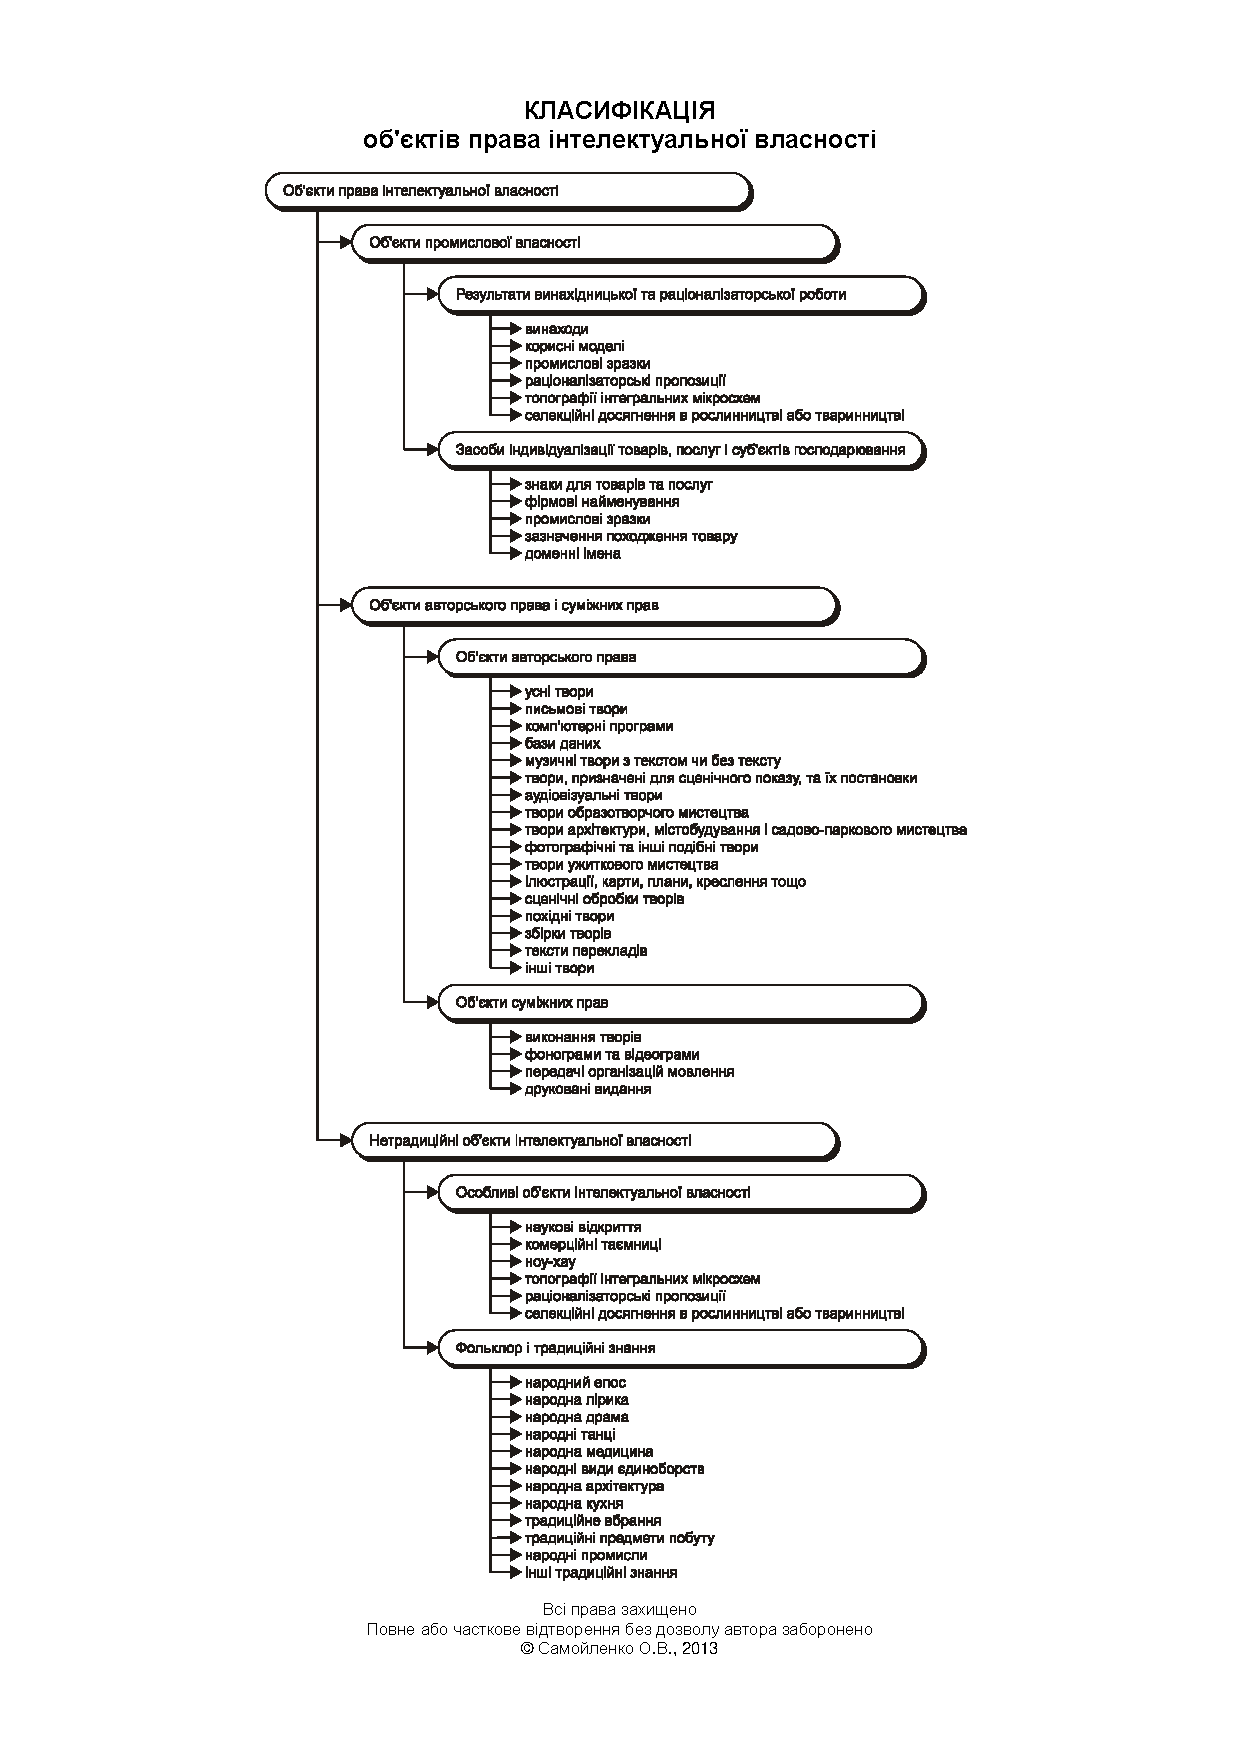
\includegraphics[scale=0.75]{opiv.pdf}
Об’єкти промислової власності названі так тому, що використовуються в основному у промисловості. Не плутати з промисловими потужностями. Головною особливістю ОПВ (об’єктів промислової власності) є те, що права на них виникають після успішного проходження ряду експертиз та виконання інших обов’язкових формальностей. 

Об’єкт суміжного права та суміжних прав. Відрізняється від ОПВ тим, що права на них виникають автоматично за фактом створення твору. І для виникнення прав не обхідно жодних формальностей.

% !TeX spellcheck = uk_UA
\subsection{Суб’єкти} 
\textbf{Суб’єктами права} можуть бути автори або інші особи, яким можуть належати майнові права на ОПІК.

\textbf{Автор} - це завжди фізична особа або група фізичних осіб. Особа автора є первинною і саме від нього походять всі майнові та немайнові права. 

Майнові права можуть належати автору, роботодавцю, покупцю, спадкоємцю, обдарованому і так далі.

Після закінчення терміну дії охоронного документа або закінчення терміну правової охорони, майнові права зникають і ОПІВ стає суспільним надбанням. Тобто, його може використовувати будь-хто, але привласнити його собі не може. 

\subsection{Законодавство у сфері ІВ}
\subsubsection{Вітчизняне законодавство}
Вітчизняне законодавство можна умовно розділити на загальне та спеціальне.  

До загального законодавства відносяться: Конституція України (4 статті), Кодекси(9 штук): по перше Цивільний кодекс (книга четверта), далі Цивільно-процесуальний кодекс, Господарський і Господарсько-процесуальний кодекс, Кримінальний і Кримінально-процесуальний, кодекс законів про працю, кодекс про адміністративні правопорушення і митний кодекс. Після кодексів йдуть закони (завантажити). Останнім рівнем є підзаконні акти.

До спеціального законодавства відносяться закони України та пов’язані з ними підзаконні акти, які стосуються охорони конкретних видів ОПІВ або подоланню конкретних проблем (наприклад, недобросовісної конкуренції). Перелік законів також на сайті.

\subsubsection{Міжнародне законодавство}

При виникненні суперечок стосовно ОПІВ між резидентом України та іноземної держави, верховенство над українським законодавством мають ті міжнародні угоди, до яких приєдналась Україна і ця держава.

Його основу становлять понад 20 міжнародних угод, приблизно дві третини яких стосуються об’єктів промислової власності, а третина про авторські права та суб’єкти прав.

Ці угоди вважаються міжнародно визнаними, адмініструє ці угоди Всесвітня організації інтелектуальної власності. ВОІВ заснована була в 1967 році на Дипломатичній конференцій в Стокгольмі. З 1974 року, ВОЇВ є однією із спеціалізованих організацій ООН. До 200 країн об’єднує.

При ній діє Всесвітня академія інтелектуальної власності. Ця академія декілька разів на рік проводить курси (безкоштовні та за свідоцтвом)

Забезпечує єдині або подібні принципи охорони ОПІВ в усіх країнах-підписантах.	

Друга група угод призначення для прискорення, спрощення і здешевлення процедури отримання охорони ОПІВ одразу в декількох країнах.

Запроваджує міжнародні класифікації об’єктів промислової власності.

\subsection{Державна система правової охорони інтелектуальної власності в Україні}
Охорона ОПІВ покладена на міністерство освіти та науки. А реалізує державну політику с сфері охорони ІВ Державна служба інтелектуальної власності. Воно ще й працює над вдосконаленням законодавства. Туди входить декілька дочірніх організацій: ДП "Український інститут інтелектуальної власності" (приймає заявки на об’єкти промислової власності, проводить експертизу і виносить рішення), ДП "Українське агентство з авторських та суміжних прав" (здійснює колективне управлення правами авторів, але заявка сюди не подається), ДП "Інтелзахист" (регулює обіг контрольних марок на ОПІВ в Україні). Біля неї крутиться купа громадських організацій. 
\subsection{Набуття прав}
Права на об'єкти АП виникають автоматично за фактом завершення (правильніше - остаточного припинення) роботи над твором.
Для виникнення і здійснення прав АП не потрібно жодних обов'язкових формальностей. АП поширюється на (не)оприлюднені і (не)завершені твори. 

В будь-який час протягом терміну охорони, АП його власник або довірена особа можуть подати заяву про реєстрацію АП і отримати відповідне свідоцтво. 

В АП діє презумпція авторства - особа вважається автором, поки не доведено протилежне. У зв'язку з цим свідоцтво про реєстрацію АП не є повноцінним охоронним документом і воно може бути оскаржене і анульоване. 

Також - головний баг - АП охороняє твір лише у формі його виконання, тобто ідеї і принципи, втілені у творі, не охороняються.

Для сповіщення про свої права власник АП може використовувати спеціальне позначення, що розміщується на оригіналі та всіх копіях \textcopyright найменування автора, рік першого правомірного оприлюднення. Якщо особа автора достаменно невідома, то вважається, що особа, яка вперше оприлюднила твір, представляє інтереси автора.

\paragraph{Особливості охорони комп’ютерних програм}
Хоча формально є об’єктом АП, повинна бути захищена комплексно.
\begin{itemize}
	\item програма як така захищається як об’єкт авторського права.
	\item Алгоритм захищається патентним правом як спосіб обробки інформації - в міжнародній патентній класифікації розділ G;
	\item інтерфейс захищається як промисловий зразок. (мкпз 14-04 Комп’ютерні інтерфейси)
\end{itemize}
% а если сделать исследование по поводу лизенций opensource и украинского законодательства, на 6-м курсе не будет самостоятельных работ
\subsection{Співавторство}
Якщо твір створений кількома фізичними особами то можна говорити про співавторство при виконанні наступних 4-х умов:

/*чего-то про патологоанатомов - Юрген Торвальд "Век криминалистики"(lite) "100 лет криминалистики"(full), "Следы в пыли"*/

\begin{itemize}
	\item спільна творча праця
	\item цілісність твору (при вилученні внеску одного з авторів - твір втрачає цілісність)
	\item добровільність
	\item наявність домовленості про спільну творчу працю.
\end{itemize}

Співавторство - роздільне і нероздільне. При роздільному співавторстві внесок кожного автора є очевидним (пісня з слів та музики). При нероздільному важко або неможливо виділити внески (брати Стругацькі). При роздільному співавторстві кожен із авторів має вільне право на використання свого внеску. При нероздільному - кожен має на використання всього твору, якщо не суперечить інтересам інших. Інтерв’ю - порівну. Взагалі, авторський внесок ділиться порівну, якщо іншого не зазначено.
Якщо авторів більше 3х (внесок більше третини) - краще ухвалювати авторський договір.
При оформленні такої штуки треба слідкувати, щоб не було "загального редагування" у співавторстві. Бо тоді буде нероздільне.

\subsection{Термін дії АП}
Починає діяти з моменту остаточного припинення дії над твором. А кінцевий термін, в загальному випадку, прив’язується до смерті автора. Для зручності підрахунків прийнято, що всі фіксовані сроки відраховуються від першого січня року наступного за роком, в якому мали місце юридичні події. Особисті немайнові права оформляються безстроково. 

В загальному випадку правова охорона АП завершується через 70 років з року смерті автора (в Європи - від 50ти). Якщо твір оприлюднено анонімно або під псевдонімом, завершується через 70 років з року першого оприлюднення. Якщо особа автора не викликає сумнівів, то як в загальному випадку. Якщо твір оприлюднюється частинами, то для кожної частини терміни використовуються окремі (актуально для попереднього положення). Правова охорона твору, створеного у співавторстві, завершується через 70 років \textbf{з року (не з дати)} смерті останнього співавтора.
Правова охорона творів посмертно реабілітованих авторів завершується через 70 років після реабілітації.
Якщо твір вперше оприлюднено більше ніж через 70 років з року смерті автора, то рахується з дня оприлюднення (? неоднозначно)
Якщо твір вперше оприлюднено після терміну правової охорони, то особа, що оприлюднила твір, набуває права, подібні до авторських. Термін дії цих прав - 25 років.

\subsection{Суміжні права}
/*Свідоцтво - прив’язка реквізиту до твору.*/
Суміжні права поширюються на виконання об’єктів АП з метою донесення до кінцевого споживача. Термін СП вживається у множині тому що є ієрархія, згідно з якою кожен нижчий рівень при реалізації прав повинен враховувати інтереси всіх верхніх. Наприклад, АП належать композитору і автору слів. Виконавець повинен враховувати інтереси композитора, автора. Студія запису - автора, композитора і співака. 

Для виникнення і здійснення СП не потрібно жодних обов’язкових формальностей - виникають за фактом першого правомірного виконання твору. Термін дії - 50 років (в європах - 20 років) з року першого виконання.

Для сповіщення про свої права використовують позначення, що викоритовується (P) 
\chapter{Практика}
\section{Література}
\end{document} 
